% SET THE SCENE

% 1. Passwords are a burden for all of us, and it is getting worse. Users have a portfolio, but what is it made of and why?
As passwords remain the main authentication method on the web, users face an ever increasing challenge to select and maintain passwords. Users' strategies to mitigate this burden are often predictable, such that they use easily guessable passwords and re-use them on more than one service. If required to change a specific password, e.g. after a database breach occurred, users often simply pick another from their own password portfolio \cite{Bonneau2015ImperfectAuthentication, Florencio2014PasswordPortfoliosFiniteUser, Stobert2014PasswordLifeCycle}. How users decide among alternative passwords is a highly individual process, and it is an open question how individual predisposition of the psyche influences the decision making in these situations.
%Although the motivation for acting this way is well understood, we do not know how much of this kind of predictable behavior can be explained by looking at the user's psyche.  
%Although we have indication that passwords are maintained for a long time \cite{VonZezschwitz2013SurvivalShortest}, we know little about the influencing factors on how the actual portfolio comes to be. 


% 2. demographics and education do not explain everything about privacy attitudes, personality and GDMS are valuable.
Apart from demographic and educational factors that evidently affect password creation and coping strategies \cite{Mazurek2013Measuring}, researchers in usable security and privacy have started considering psychological variables to improve explanations for predictable user behavior. Two prominent examples for such variables are the Big-Five personality traits \cite{Goldberg1990BigFive} and the general decision making style (GDMS) \cite{Scott1995GDMS}. The Big Five model tries to characterize a person's attitudes and behavior with five distinct traits, namely openness, conscientiousness, extraversion, agreeableness and neuroticism. The GDMS model describes how people decide by classifying decision-making into rational, intuitive, dependent, avoidant and spontaneous styles. How users form privacy attitudes has been explored extensively \cite{Acquisti2005PrivacyRationality,Korff2014TooMuchChoice,Spiekermann2001EPrivacyPreferences,Woodruff2014PrivacyFundamentalist}. Egelman and Peer, however, were one of the few who suggested taking the Big-Five traits and decision making style into account to explain the preconditions for privacy attitudes \cite{Egelman2015AverageUser}. They found out that someone's decision making style is more predictive than personality traits regarding general privacy attitudes. %In this paper, we investigate if this is also true for another crucial type of privacy behavior, which is to judge the strength of passwords. 

% 3. creating a password is also a decision making process. 
% 4. password strength perceptions have been explored for average users, but where are the individual differences? 
%    --> why are the individual differences necessary?
%    --> why do we think that the differences could result from personality or decision making style?

Decision-making tasks can also be found in password selection: When a user is required to create a password, he or she can either come up with a new one by combining letters, digits and symbols or pick an old password from his or her personal portfolio that usually consists of around five distinct passwords \cite{Florencio2007LargeScaleStudyPasswordHabits}. In any case, the outcome of this decision-making process depends on evaluating ease of typing, memorability, or the perceived strength. When users judge the strength and memorability of passwords, they do this in predictable ways \cite{Ur2016PerceptionsPassword}. They often base their judgment on the variety of characters forming the password. Although there are indeed certain themes in the way users perceive strength, the perceptions are not shared unanimously among all users. Examining what causes the discrepancies is important to help users better understand password strength and to design usable support systems. We hypothesize that the perception of password strength may be influenced by variables like personality traits or decision making style. 

In this paper, we investigate the associations between the Big-Five personality traits, general decision making style and users' perceptions of password strength. In an online study with 100 participants, we administered psychometric tests and collected subjective strength ratings of diverse passwords. We examined the associations between the psychometrics and password strength ratings. Among our key findings, we observed that respondents with high openness scores were more skeptical than the rest about the strength of passwords shown in the study. Moreover, those who score high on conscientiousness were more likely to compare two given passwords by the variety of characters. Rational decision makers performed significantly worse in identifying the stronger of two given passwords.



\section{Background and Related Work}
\subsection{Password Strength Metrics}
%First of all, strong passwords are desirable to protect personal information, 
%TODO motivation: Why do we need strong passwords? Do they achieve anything?
%TODO wir brauchen noch den Hinweis, dass z.B. Substitutionen oder erratbare Modifikationen nicht viel bringen. 
%\subsubsection{Metrics}
Finding an objective and reliable measure for the strength of a given password is difficult. The NIST-entropy of a password is a standard and commonly used measure. It reports the degree of randomness of the characters inside a password \cite[ Appendix A therein]{Burr2011NIST}. However, as more advanced threat models emerged, more realistic measures were proposed. In offline-attack scenarios, the entire database containing the passwords as hashes is obtained by the attackers, which happens sporadically even with highly frequented services like LinkedIn \cite{Florencio2007DoStrongWebPasswords,Scott2016ProtectingLinkedIn,Shay2016DesigningPasswordPolicies}. This means attackers can try millions of times to guess passwords and their efforts are only limited by time and computing power. Multiple researchers proposed that the number of guesses required to crack a password is often a more accurate metric for strength \cite{Kelley20012GuessAgain, Shay2016DesigningPasswordPolicies, Weir2010MetricsPolicies}. Carnegie Mellon University has established a Password Guessing Service (PGS) that allows uploading a list of passwords and receive success rates from various cracking approaches \cite{Ur2015MeasuringRealWorldAccuracies}. To use the service, however, the passwords need to be collected and uploaded in clear-text. This is not always possible in password studies, mostly for ethical reasons. There are other means to estimate the required number of guessing attempts. For example, the zxcvbn algorithm shows high accuracy up to one million guesses, which is a realistic cut-off threshold for online attacks \cite{Wheeler2016zxcvbn}. It can be implemented as a lightweight script and is easy to include in pro-active password checks.


\subsection{Human Factors in Password Strength}
Leaked data from real-world accounts has repeatedly shown that user selected passwords are often predictable \cite{Bonneau2012ScienceOfGuessing}. Given the freedom to select any password, many people opt for simple, short, memorable words or numbers that are easy to type. Because such passwords are vulnerable to informed guessing attacks, service providers try to prevent them by introducing a set of requirements to reduce the risk of account hijacking. However, such composition policies are not implemented identically on all web services \cite{Wang2015EmperorsPolicies}. Often, when users create an account, they re-use a password from elsewhere \cite{Das2014TangledWeb}, which is sometimes prevented if policies differ in requirements. Users then often modify the password until the requirements are met \cite{Inglesant2010TrueCostOfUnusablePolicies,Komanduri2011OfPasswordsAndPeople}. The resulting passwords do not necessarily gain strength, if they are only appended by digits or symbols at predictable positions \cite{Weir2010MetricsPolicies}. Thus, balancing the demands in terms of usability and security of a password policy is challenging and has been under constant research in the past few years \cite{Melicher2016UsabilityMobileTextPasswords,
	Shay2016DesigningPasswordPolicies, 
	Shay2014CanLongPasswordsBeSecureAndUsable,
	Wang2015EmperorsPolicies}. One important aspect of password policies that possibly affects how users evaluate password strength is their educational effect. Users are often exposed to requirements that do not necessarily lead to stronger passwords. The length of the password is often more crucial for the strength than character diversity. For instance, when policies require three different character classes with minimum length twelve (3class12), user-selected passwords are often more guessable than those created with a simple length requirement of 16 characters (basic16) \cite{Shay2014CanLongPasswordsBeSecureAndUsable}. At the same time, users are being told that character variety is necessary to form strong passwords \cite{Ur2012HowDoesYourPasswordMeasureUp}. The long-term consequences are that users sometimes have a suboptimal perception of the factors that add to the objectively measurable strength of a password \cite{Ur2016PerceptionsPassword}. %To this point, psychological factors affecting the susceptibility to educational effects of password policies are underexplored, which we try to   
%HH: Das könnte man mit einem Beispiel unterstützen. Ich denke, das klassische Beispiel ist, dass die Länge wichtiger ist als ob eine Zahl vorkommt.



Beside the constraints dictated by composition policies, many users have developed coping strategies for handling authentication tasks \cite{Stobert2014PasswordLifeCycle}. For example, the value of an account is decisive whether users pick a strong or weak password from their portfolio. Stobert and Biddle argue that this process is deliberate and even IT experts are prone to choose weak passwords for accounts that they do not deem worthy to protect  \cite{Stobert2015ExpertPassword}. Flor\^{e}ncio and Herley argue that this behavior is rational from an economics and efficiency perspective \cite{Florencio2014PasswordPortfoliosFiniteUser}. Still, if users receive security advice by trusted peers, they might reconsider behaviors like password re-use \cite{Das2014EffectSocialInfluenceSecuritySensitivity}.


It was also shown that nudging is effective to make users try and increase password strength. Presentation effects of the nudges can play a role. For example, the design of a password meter can impact how much effort users put into the creation of the password \cite{Ur2012HowDoesYourPasswordMeasureUp}. If shown suggestions, participants in a controlled online study created stronger passwords depending on the kind and number of suggestions \cite{Seitz2016SuggestionsDecoy}. Another intrinsic factor is the degree and type of exposure to social influence in the form of stories or advice. Das et al. showed that such advice affects the intrinsic motivation of acting more secure on the web \cite{Das2014EffectSocialInfluenceSecuritySensitivity}. 

The participants' meta password characteristics are important to find out if past actions influence strength ratings. The participants reported to use passwords that were nine characters long ($Md=9,~SD=3$), which is consistent with the finding that most real-world policies require a minimum of eight or nine characters \cite{Wang2015EmperorsPolicies}. The medians for other password characteristics were 1 uppercase letter ($SD=1$), 2 digits ($SD=3$), 0 special characters ($SD=1$) and 1 dictionary word ($SD=1$).

%\subsubsection{Behavior and Strength Rating}
Before we analyzed the influence of personality traits on the ratings, checked associations between meta passwords and password ratings. We performed linear regression analyses as shown in Table \ref{tbl:personalpw_regression}. The regression models reveal that ratings were mostly associated with the length and usage of uppercase letters inside one's own password. Model fit was $R^2_{adj}=0.12$ for overall rating. Particularly in the second row of Table \ref{tbl:personalpw_regression}, we can see that participants, who report to include more uppercase letters in their meta passwords, were more likely to give lower overall strength ratings (cf. Figure \ref{fig:MetaPW-ViolinPlot}). Regarding the comparison task, we found that the meta passwords were only very weakly associated with the outcome (mean $R^2_{adj}=0.03$). Hence, we do not present detailed statistics. 


% Table generated by Excel2LaTeX from sheet 'Correlation Matrix SLUDS'

\begin{table}%[htbp]
  \centering
  \small
  \caption{Regression analysis with participants' proxy password characteristics as independent variables and ratings for password groups. Especially the use of uppercase letters is negatively correlated with the ratings. Numbers in bold indicate statistical significance ($p<0.05$)}
  \resizebox{\linewidth}{!}{
\begin{tabular}{l|r|rr|rrr|rrr}
    \multicolumn{1}{c|}{\multirow{2}[1]{*}{\textbf{Proxy PW Characteristic}}} & \multicolumn{9}{c}{\textbf{Password Ratings}} \\
      & \multicolumn{1}{c|}{Overall} & \multicolumn{1}{l}{Long} & \multicolumn{1}{l|}{Short} & \multicolumn{1}{l}{Weak} & \multicolumn{1}{l}{Medium} & \multicolumn{1}{l|}{Strong} & \multicolumn{1}{l}{Special} & \multicolumn{1}{l}{Digits} & \multicolumn{1}{l}{Uppercase } \\
    \midrule
    \rowcolor[rgb]{ .922,  .945,  .871} Length & -0.13 &   & -0.12 & \textbf{-0.20} &   &   & \textbf{-0.21} &   & -0.13 \\
    \rowcolor[rgb]{ .922,  .945,  .871} Uppercase Letters & \textbf{-0.33} & \textbf{-0.31} & \textbf{-0.26} &   & \textbf{-0.37} & \textbf{-0.25} & -0.18 & \textbf{-0.41} & \textbf{-0.30} \\
    \rowcolor[rgb]{ .922,  .945,  .871} Digits &   &   &   &   &   &   &   &   &  \\
    \rowcolor[rgb]{ .922,  .945,  .871} Symbols &   &   &   &   &   &   &   & 0.12 &  \\
    IT Background &   &   &   & -0.10 &   &   &   &   &  \\
    Education &   &   & 0.11 &   &   & -0.12 &   &   &  \\
    Gender &   &   &   &   &   &   & 0.20 &   & 0.10 \\
    \midrule
    \textbf{F} & \textbf{7.64} & \textbf{10.29} & \textbf{3.74} & \textbf{3.27} & \textbf{15.33} & \textbf{3.89} & \textbf{3.40} & \textbf{9.45} & \textbf{4.13} \\
    \textbf{p} & 0.00 & 0.00 & 0.01 & 0.04 & 0.00 & 0.02 & 0.02 & 0.00 & 0.01 \\
    \textbf{Adj. $R^2$} & \cellcolor[rgb]{ .675,  .831,  .502} 0.12 & \cellcolor[rgb]{ 1,  .922,  .518} 0.09 & \cellcolor[rgb]{ .992,  .812,  .494} 0.08 & \cellcolor[rgb]{ .973,  .412,  .42} 0.04 & \cellcolor[rgb]{ .592,  .804,  .494} 0.13 & \cellcolor[rgb]{ .976,  .545,  .443} 0.06 & \cellcolor[rgb]{ .988,  .702,  .475} 0.07 & \cellcolor[rgb]{ .388,  .745,  .482} 0.15 & \cellcolor[rgb]{ .992,  .922,  .518} 0.09 \\
    \bottomrule
    \bottomrule
    \end{tabular}%
        }
%  \resizebox{\linewidth}{!}
%{
%
%
%}
  
  \label{tbl:personalpw_regression}%
\end{table}%

%In the first phase of the study, the participants were asked to imagine their email provider required them to create a new password and they could not select their current one. This measurement was taken early to prevent bias from showing different types of passwords. The answers were collected in plain text. We proceeded to have the users choose the type of account that they would be willing to secure with their selected password in the real world. This would indicate the effort and the value of their selection.


%we need to be aware that a more faceted personality profile may reveal larger differences. 
%TODO viele antworten deuteten darauf hin, dass englisch nicht in die muttersprache ist. 
%TODO meta password characteristics are not an accurate proxy for password strength, as depicted in the background section. 
%Our proxy for password strength is the result of the zxcvbn estimator algorithm \cite{Wheeler2016zxcvbn}. While it can estimate the strength of passwords in attack scenarios up to one million guesses, its estimates become more fuzzy above this threshold. However, for the purpose of the study, the estimate was considered good enough as it still highly correlates with the estimates of more sophisticated tools like the password guessing service (PGS) \cite{Ur2015MeasuringRealWorldAccuracies}. 
%\begin{itemize}
%\item we might measure intelligence
%\item self-reporting might not be accurate
%\end{itemize}


%As we collected plain text passwords that could -- in theory -- be linked backed to an individual, we took special care to point out that participants should not enter their actual password, but to think of a new one. The additional meta characteristics are most likely insufficient to reconstruct a participant's actual password. 

%\begin{figure}
%	\centering
%	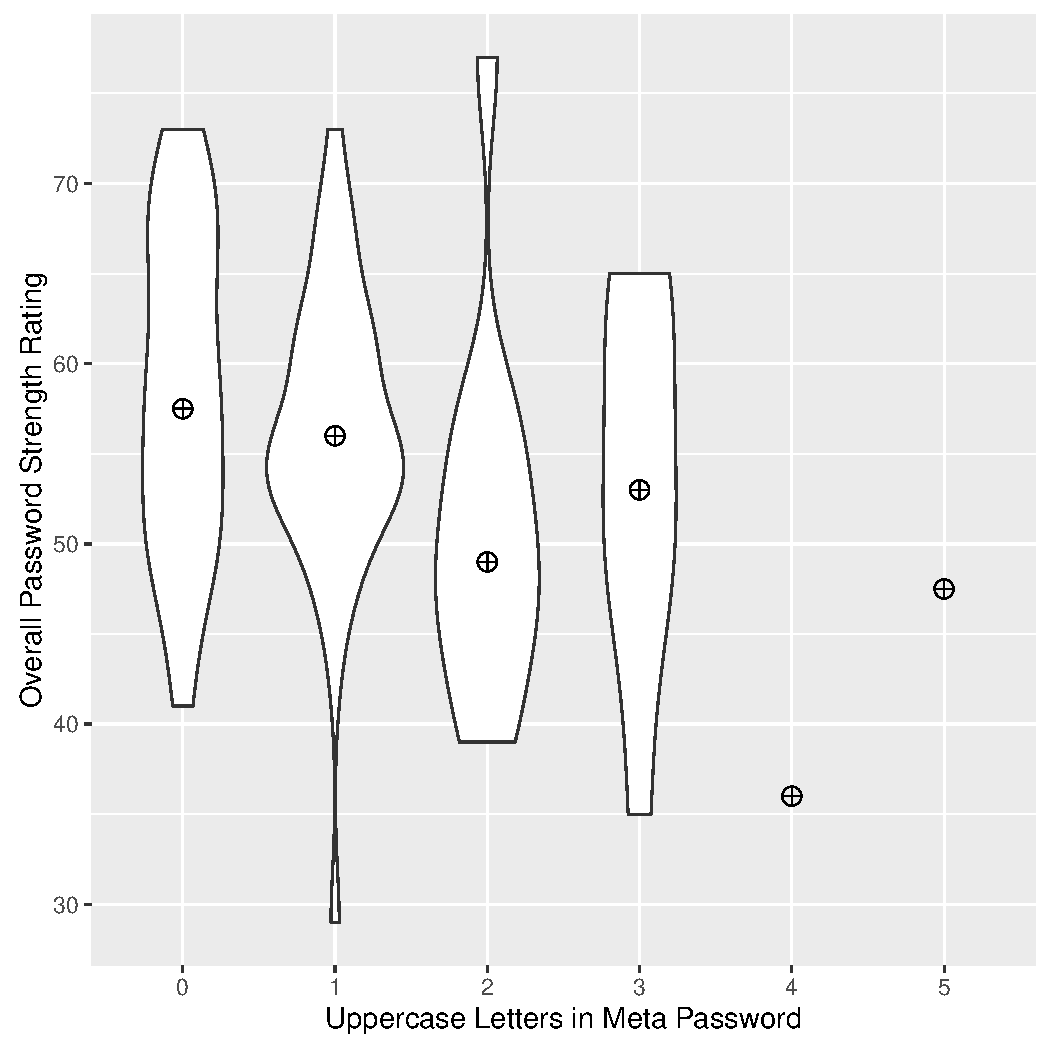
\includegraphics[width=\linewidth]{figures/MetaPW-Violinplot}
%	\caption{\label{fig:MetaPW-ViolinPlot} Violin plot of strength ratings, grouped by the number of uppercase letters in the participants' meta password. The plot gets broader, the more respondents scored in the particular range. The plot shows a negative association between overall password strength and uppercase letters in the meta password.}
%\end{figure}
%Table \ref{tab:Regression-Rating} shows the regression results of standalone password ratings. The overall ratings in the first column, which we consider the most important metric, were negatively associated with the \textit{openness} trait ($\beta = -0.25, p < 0.05$) (see also Figure \ref{fig:openness-scatterplot}). In other words, participants with higher openness scores were generally more pessimistic regarding password strength, which was also the case if participants had a technical background, albeit this association was not as strong. Higher agreeableness scores were slightly associated with more optimistic overall password ratings. Interestingly, with conscientiousness and extraversion, two of the big-five factors never played a significant role and thus are omitted in Table \ref{tab:Regression-Rating}.


%The decision making style predictors were retained in four of the nine models, but never showed high predictive power. Contrarily, the openness trait was retained in the regression models across the board. For example, especially the weaker passwords receive lower ratings from people with higher openness scores. However, the average adjusted $R^2$ across all categories tells us that the models explain only a rather small portion of the variance in the password ratings ($M=0.06~(SD=0.03)$). 

%The lower half of Table \ref{tab:B5-Regression-Comparison} shows the analysis results for standalone password ratings. One can see that there were no striking associations between predictors and dependent variables. Also, the models with the highest $R^2$ value needed six degrees of freedom on average. This means that no particular decision making style stands out to inform the predictions. The maximum $R^2$ value across the models here is $0.05$, i.e. very low. Thus, decision making style did not explain variances satisfactorily.
\begin{figure}
	\centering
	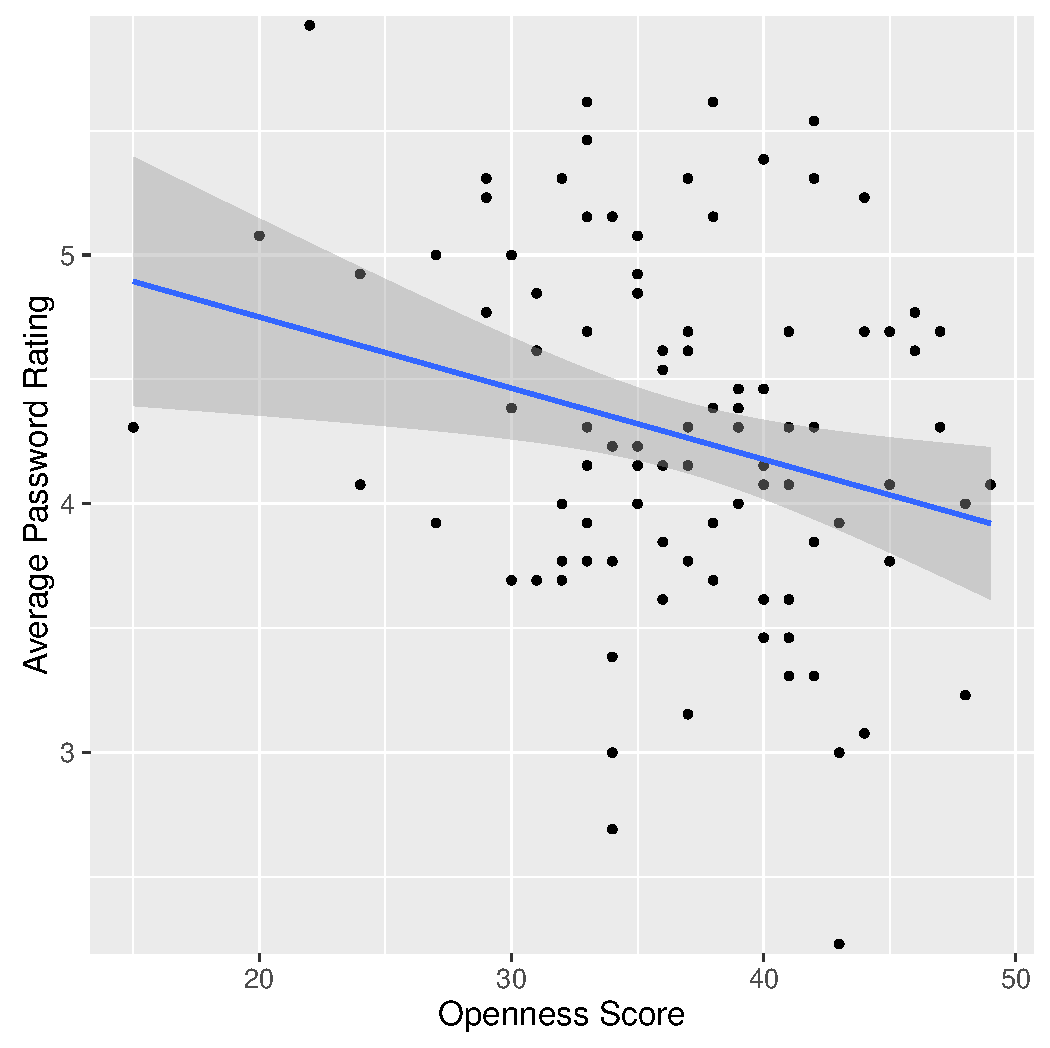
\includegraphics[width=\linewidth]{figures/Openness-ScatterPlot3}
	\caption{\label{fig:openness-scatterplot} Scatter plot of openness scores on x-axis and overall password ratings on y-axis, with fitted regression line and 95\% confidence interval. Participants scoring high on openness are a little more pessimistic in rating the strength of passwords.}
\end{figure}


We also see moderate associations between decision making style and the evaluation based on length and strength as measured by zxcvbn. There is a noteworthy finding concerning people ranking high on rational or intuitive decision making style. We find that rational decision makers were worse at identifying the stronger password ($\beta = -0.35, p < 0.01$) than the intuitive decision makers ($\beta = -0.18, ns$).  

\subsection{Big Five Traits vs. Decision-Making Style (RQ2)}
We initially posed the question whether the Big-Five Model or the General Decision Making Style is better at predicting how users evaluate passwords. This question is difficult to answer with our current results. In absolute terms, the Big-Five variables more often boosted predictive power, but this alone is not sufficient to prefer them to GDMS. As discussed above, openness and conscientiousness were the strongest predictors of the Big-Five model, while the rest was largely insignificant. For the GDMS, the rational and intuitive dimensions showed noteworthy associations. It appears the question is not, whether one scale is better than the other, rather than what can be gained by combining them, and for what kind of scenario it makes sense to do so. 

For the standalone rating, adding the predictors from the GDMS fails to increase predictive power. The model fit can be achieved with the Big-Five factors alone, because the fit is low in any case. However, this is not the case when predicting the outcome of deciding which one of two given passwords is stronger. Here, the models became better if the GMDS factors were added. Likewise, sticking to GDMS and omitting predictors from the Big Five model is also suboptimal for the comparison task, because we lose much of the predictive power. 

We conclude that the origin of this finding must be in the nature of the task. Rating one password without an anchor seems more difficult, and thus it is probably easier for open people who are good at solving difficult problems. On the other hand, if there is a second password, the decision seems to trigger additional mental processes to solve the task and is easier for people who have static mental models about password strength characteristics. Intuitive decision makers were less likely to fail at spotting the stronger password than rational decision makers. It looks as if the decision is rational, but not objective, or that the rational deciders ``overthink'' their assessment. 

\subsection{The Role of Our Own Passwords (RQ3)}
Respondents' meta-passwords also showed some predictive power for password ratings. However, they were basically not associated with the outcome of the comparison task. %Especially participants who use more uppercase letters in their own password(s) gave lower strength ratings. 
Although we can only speculate, participants may possibly have compared the study passwords to their own password only during the rating task. Hence, characteristics from their own password may have become more salient, e.g. the use of uppercase letters. Once they saw two passwords on the screen during the comparison task, their own baseline might have turned less important. This would substantiate that the scenario -- standalone rating or comparison -- is really the key to get the full picture of password perception. %If this were the case, looking at the influence of psychological factors in the two tasks separately is even more necessary. 

Moreover, users keep a portfolio of passwords that differ in strength, and they use their stronger passwords on high-value accounts \cite{Egelman2013DoesMyPasswordGoUpToEleven,Florencio2007LargeScaleStudyPasswordHabits}. This implies that users have a couple of ``weak'' passwords, but still consider them suitable in some situations, e.g. when they do not believe they need the account again. Our qualitative analysis, however, found no evidence of participants mentioning this factor when evaluating the strength of the given passwords. None of them mentioned judging the strength of the passwords in regards to what they are meant to protect. Thus, we conclude another kind of scenario may be necessary, in which the evaluation also takes the usage context into account.






%\subsection{RQ1: Traits of Password Strength Perception}
\subsection{The Weight of Openness and Conscientiousness}
%1. interpret negative correlation between openness and password rating
The passwords in our study received lower strength ratings from people with high openness scores, i.e. those who would describe themselves as creative, imaginative, intelligent or liberal. %At the same time, the meta passwords of these participants were similar to those of other participants. The effect thus only seems to concern the \textit{perception} of password strength -- not personal behavior. 
Looking for an explanation for these observations, we could attribute them to the ``divergent thinking'' facet exhibited by people with higher openness scores \cite{McCrae1987DivergentThinking} as well as the association with general intelligence \cite{DeYoung2015}. In this sense, participants with higher scores in openness could have been more likely to discover patterns in passwords due to higher creativity and cognitive abilities. A cue for this interpretation is P21's description of his approach: 
\begin{quote}
	\textit{``If it looked like dictionary passwords I rated it lower, more random unrepeated ones rated higher. Combinations of words also scored higher''}
\end{quote}
There were only few participants (6) who mentioned word combinations as beneficial for password strength. This diverges from the more commonly mentioned theme that dictionary words are bad for password strength. Accordingly, an explanation for the diverging assessment by participants with higher openness scores lies in the problem-solving skills that are usually attributed to more open people \cite{DeYoung2015, McCrae1987DivergentThinking}. The tasks we picked for our study are indeed problems that can be solved by relying on objective criteria. It is thus very likely that those participants took a more objective, albeit critical stance when rating the strength of the passwords. They correctly identified that password length is usually more important than the inclusion of digits. 

%2. interpret positive correlation with conscientiousness and LUDS
% policies have primed people too much and  
In contrast, conscientious participants were more likely to compare passwords by their variety of characters instead of length. It seems that they diligently check off an imaginary list of criteria that a strong password needs to have, just like when users face requirements dictated by policies.  Although much research has gone into optimizing password policies for a general audience, the recommendation of the 2word16 policy over more complex ones \cite{Shay2016DesigningPasswordPolicies}, for example, has not been implemented at scale in practice, yet. Instead, policies for the most part demand the inclusion of different character classes \cite{Wang2015EmperorsPolicies}. Our data suggest that conscientious participants, who are characterized as being more scrupulous and neat, are more likely to look out for details about character classes when they judge the strength of a password. Thus, we assume that conscientious participants benefit from having such a list of requirements dictated by policies and that they would not easily adopt policies demanding words instead of character diversity.
%The exposure to this type of policies might be the main reason why many participants in our study penalized passwords that contained words or that were in some ways meaningful.

We reason that managing passwords, i.e. \textit{creating}, \textit{committing to} and \textit{coping with} them \cite{Stobert2014PasswordLifeCycle}, is a problem that is more easily solvable for people with open minds or a disposition to treat the problem with diligence. It is less affected by their leaning towards agreeableness, extraversion, or neuroticism. So, we reason that password strength as an objective measure is also associated with the personality traits that are informed by objectivity. In that sense, the regression models understandably benefited from openness and conscientiousness.




\section{Implications for Research and Design} \label{sec:implications}
From the discussed points, we would like to point out where the findings have immediate and indirect implications. 

\subsection{Assessing Personality Traits in Password Studies}
Studying passwords is challenging, because we often lack access to real-world testbeds. Thus, online studies are the go-to method, which is usually reliable. However, the modification of independent variables in these online studies may not be the sole cause of effects. Confounding variables beyond demographic questions are seldom considered. Psychometrics may come in useful to evaluate causal relationships, however, they are to this date often neglected. We have shown that they have explanatory value and thus should not be neglected, if we want to stop designing security mitigations for the ``average user'' \cite{Egelman2015AverageUser}. 

However, including elaborate psychometric tests in addition to the core of the research question is probably unrealistic. Thus, to keep studies short and prevent participant fatigue, we propose to focus on the openness and conscientiousness personality traits. These can be measured with a bare minimum of 20 items, so they do not take more than five minutes to answer. If the scenarios in the password study resemble our comparison task, it is potentially viable to also include assessments on rational and intuitive decision making. 

Still, adding more items to a questionnaire might not always be possible. There is, however, a promising approach to quickly and inexpensively obtain personality data from study participants' past behavior. It is possible to infer personality facets from social media data, e.g. the number of friends on Facebook or public interactions \cite{Youyou2015Personality}. Youyou et al. found that such metrics can even outperform psychometric questionnaires. We thus suggest to request permission to access information that participants made available on such platforms and run personality analyses on the anonymized versions of it. Requesting permission to install software on mobile devices for research purposes has received little concern with crowd-workers in a large-scale study by Bentley and Chen \cite{Bentley2015Phonebook}. While we would not go so far as to read all contacts, call and message history, we believe a privacy sensitive version of this approach can replace personality tests.

\subsection{Password Suggestions}
Addressing personality facets might also become beneficial for real-time feedback during password creation. In the wild, we encounter password meters that estimate the strength of the password and in some cases even provide verbal feedback about what the user can do to improve the password (e.g. \cite{Wheeler2016zxcvbn}). A simple approach is to try and convince the user to pick a stronger password by suggesting a new one or a modified version of the entered password \cite{Forget2008ImprovingPasswordsThroughPersuasion, Seitz2016SuggestionsDecoy, Shay2015SpoonfulOfSugar}. 

Coming back to the finding that personality has an effect on how people \textit{compare} two passwords, we suppose that it plays a role for real-time suggestions, too. How a modified version or newly generated password is received likely depends on the user's personality. For instance, if the user's password is visible in clear text while they enter it, adding a suggestion next to the password results in a scenario similar to the comparison task from our study. Then we can conclude that it would be easier for conscientious people to assess the strength of their password, if there is a clear list of requirements than can be ``checked off'', to make it superior to the suggested password. Moreover, users with high openness trait characteristics might make their password longer if they see the suggested password is much longer than their own. The results from Seitz et al. point in this direction, because their study participants picked longer passwords, if a long password was suggested \cite{Seitz2016SuggestionsDecoy}. We reason that the approach could have produced larger effect sizes, had the participants' personality been taken into account and had the password been displayed in plain text. Similarly, user acceptance suffered in Shay et al.'s modification approach, maybe because it was not tailored to individual users \cite{Shay2015SpoonfulOfSugar}.

%\begin{itemize}
%\item there have been attempts to convince users of stronger passwords by simply suggesting new ones or alterations of the existing passwords \cite{Forget2008ImprovingPasswordsThroughPersuasion, Seitz2016SuggestionsDecoy, Shay2015SpoonfulOfSugar}. 
%\item If the user's password is visible during selection (a scenario most often useful on mobile devices \cite{Melicher2016UsabilityMobileTextPasswords}, this could make them compare the strength 
%\item there's a question if the users can stay neutral enough to re-evalute their own password 
%\end{itemize}


% DESIGN Space. Problem solving or not? 
\subsection{Personalized Password Policies}
Our results indicate that users have different, sometimes sophisticated approaches when they evaluate password strength, which is in line with related work \cite{Ur2016PerceptionsPassword}. The origin of these approaches is not directly linked to personality, but personality traits may influence what users pay attention to when they face password policies. Diligent users could look out for and remember a list of requirements, while only the minimum length is important for creative minds. Identity providers like Facebook or Google rely on passwords to authenticate users and currently implement a ``one-fits-all'' password policy. However, once users have used the services for a while, those parties already possess a large amount of user information. Consequently, the identity providers could alter the enforced policy for individual users depending on personality trait characteristics inferred from usage patterns. We propose to dynamically adjust the policy, for example when users reset their password. Conscientious users may welcome a more complex policy,  e.g. 3class12 (cf. Shay et al \cite{Shay2016DesigningPasswordPolicies}), while others create passwords with a 2word16 requirement. Such approaches could reduce user frustration and boost usability. 

%%TODO identity providers.
%\begin{itemize}
%\item our results indicate that users have different approaches to evaluating passwords
%\item since we see interactions with personality, we hypothesize that their personality influences what they
%take from password policies (e.g. what they can remember, or what they believe). 
%\item we cannot adjust / personalize password policies for unknown users
%\item we can personalize policies for password resets, because we already have some data about the user
%and it can be used to inform personality assessment.
%\item is the policy presented
%
%\end{itemize}


%Considering that people's personality is a factor that affects the perception of password strength, this directly leads to the question about how we can address personality in current password policies. The policies put a high burden on users and their effect is controversial. Thus, we could try and make password policies more usable by the framing them to better reach the right audiences in the right ways, rather than using ``one fits all'' approach. Of course, at the moment of password selection, a service does not know the user yet and thus lacks information on their personality. However, the problem might be solvable on mobile devices, where the usage patterns let us already draw conclusions about the user's personality \cite{Oliveira2011Psychographics}. The idea of adjusting password policies depending on the device on which the password is created has also been put forward recently \cite{Melicher2016UsabilityMobileTextPasswords}. It thus seems beneficial to investigate how to bring the two concepts together. 